\subsection{A uniform annular lower bound}
\label{sec:annular-bound}

Let \(r_0=\sqrt{3/2}\), \(\rho=5/4\), \(R=2r_0\), and
\(q=\sqrt{8/5}\). Write \(B_t\) for the ball of radius \(t\) about
the centre \(0\). Let \(Y\) be all other centres of norm less than \(R\).
Define the annular volume left by those centres as
\[
 A(Y)=\vol\bigl(V(Y)\cap(B_\rho\setminus B_{r_0})\bigr).
\]
The previous truncation has volume
\(T(Y)=\vol(V(Y)\cap B_{r_0})\).
For \(r_0\le t\le q\), put
\[
 g(t)=2\pi\frac{(q-t)^4}{(q^2-1)^{3/2}} .
\]

\begin{thm}[Annular volume and exterior cuts]\label{thm:annular-bound}
For every packing of unit balls in four dimensions and every centre,
\[
 \vol\bigl(V_0\cap(B_\rho\setminus B_{r_0})\bigr)
 \ge \frac{77}{100} A(Y),\qquad
 \vol V_0\ge T(Y)+
 \max\left\{g(r_0),\ \frac{77}{100}A(Y)+g(\rho)\right\}.
\]
Moreover \(g(r_0)>1/28600\). In particular the cell has volume greater
than \(8\) whenever \(T(Y)\ge 8-1/28600\).
\end{thm}

\begin{proof}
\emph{Exterior cuts.}
An exterior centre \(z=su\) can cut positive volume from \(B_\rho\)
only for \(R\le s<2\rho\), with \(u\) unit. For \(y=dv\in Y\), with
\(v\) unit, separation gives
\[
 u\cdot v\le \frac{s^2+d^2-4}{2sd}\le \frac d5+\frac{9}{20d}.
\]
The second inequality substitutes \(s=5/2\), since the first
right-hand side is increasing in \(s\) on this range. Let \(b=1/4\)
and let \(\alpha_d=\arccos(2d/5)\), the angular radius of the cap
cut by \(y\) on the sphere of radius \(\rho\). We claim
\[
 \cos(\alpha_d+b) > \frac d5+\frac{9}{20d}.
\]
Indeed the derivative of the left-hand side with respect to \(d\)
is at least \((2/5)\cos b>1/5\), by expanding
\(\cos(\alpha_d+b)=(2d/5)\cos b-\sqrt{1-4d^2/25}\sin b\).
The derivative of the right-hand side is at most \(1/5\).
At \(d=2\) we have
\((4/5)\cos b-(3/5)\sin b>5/8\), by
\(\cos b\ge 31/32\) and \(\sin b<b\). This proves the claim.
It follows that every direction within \(b\) of \(u\) is outside
every cap from \(Y\) at radius \(\rho\). It stays outside those caps
at smaller radii.

For two exterior centres capable of cutting \(B_\rho\),
the analogous upper bound on their directional inner product is
\(17/25\), obtained by replacing both radii by \(5/2\).
The expression is increasing in both radii because their squared
values lie in \([6,25/4]\). Since \(\cos(2b)\ge7/8>17/25\),
the angular caps of radius \(b\) about their directions are disjoint.
Thus each exterior centre reserves a disjoint sector in the volume
\(A(Y)\), whether or not it cuts any of that volume.

The spherical cap of angular radius \(b\) in \(S^3\) has area
\(C(b)=4\pi\int_0^b\sin^2 w\,dw\).\footnote{In the parametrisation
\((\cos w,\sin w\,\omega)\) with \(\omega\in S^2\), the angular
area factor is \(\sin^2 w\), and \(S^2\) has area \(4\pi\).}
Its sector between \(r_0\) and
\(\rho\) has volume at least
\[
 L=r_0^3(\rho-r_0)\frac{4\pi}{3}\left(\frac{95}{96}\right)^2 b^3 .
\]
Here \(\sin w\ge w-w^3/6\ge(95/96)w\) for \(0\le w\le b\).
By perpendicular sections, an exterior centre cuts at most
\[
 \frac{4\pi}{3}\int_{r_0}^{\rho}(\rho^2-h^2)^{3/2}\,dh
 \le \frac{8\pi}{15}(2\rho)^{3/2}(\rho-r_0)^{5/2}.
\]
The ratio of the last expression to \(L\) is smaller than
\(23/100\), as verified by rational inequalities in
\cref{app:annular-constants}. If there are \(N\) exterior centres
with \(s<2\rho\), then \(NL\le A(Y)\). The removed annular volume
is therefore at most \((23/100)A(Y)\). This proves the first
inequality.\footnote{An exterior centre at exactly \(2\rho\) cuts
zero volume. No assumption on the shape, order or symmetry of \(Y\)
is needed.}

\emph{Volume beyond a sphere.}
First arrange that the cell is bounded without changing its shell.
If necessary, add centres on the sphere of radius \(R\) until no
further centre can be added there. This takes finitely many steps,
since the added centres are \(2\)-separated on a compact sphere.
Every point of that sphere is now at distance strictly less than
\(2\) from some centre other than \(0\). The augmented cell is
contained in \(B_R\) by convexity. It is a polytope, since only
finitely many centres can affect the inequalities inside \(B_R\).
For instance, the finitely many centres with norm at most \(2R\)
already exclude the entire sphere of radius \(R\).
The augmentation leaves \(Y\) and \(T(Y)\) unchanged.

At any vertex \(p\) of the bounded cell there are at least four
active neighbours. Take four of them with \(0\). These five points
are pairwise at distance at least \(2\), and all lie at distance
\(|p|\) from \(p\). Writing \(\bar y\) for their centroid, the sum
of their squared pair distances equals
\(5\sum_i |y_i-\bar y|^2\le 25|p|^2\).
The sum is at least \(40\), so \(|p|\ge q\).

Choose a maximal subset of vertex directions \(p/|p|\) at pairwise
angular distance at least \(1/10\). For each unit vector \(w\) there
is a vertex \(p\) with \(w\cdot p\ge1\), since the cell contains
the unit ball. Its direction is at angle at most \(\arccos(1/R)\)
from \(w\), and there is a selected direction within \(1/10\) of it.
The cosine of \(\arccos(1/R)+1/10\) is at least
\((199/200)/R-1/10>1/4\), using \(R<5/2\).
The convex hull of the selected directions thus contains a ball
about the origin of radius strictly greater than \(1/4\).
There are at least six selected directions.\footnote{If there are
at most five, the full-dimensional hull must be a simplex.
Write the origin as a positive barycentric combination of its five
vertices. Some weight \(\lambda\) is at most \(1/5\).
In the direction normal to the opposite facet, the corresponding
vertex has inner product at least \(-1\). The barycentric identity
therefore bounds the distance of that facet from the origin by
\(\lambda/(1-\lambda)\le1/4\).}

For each selected direction \(e\), the cell contains \(qe\) and
the unit ball. It therefore contains the cone joining \(qe\) to
the unit ball's section in the plane \(x\cdot e=1/q\).
At axial height \(h\in[t,q]\), the cone section is a three-ball
of radius \((q-h)/\sqrt{q^2-1}\). All points of these sections are
at angular distance less than \(1/20\) from \(e\), by
\((q-r_0)/(r_0\sqrt{q^2-1})<1/20\) from
\cref{app:annular-constants}. Hence the portions from different
selected directions are disjoint. Their volumes sum to at least
\[
 6\frac{4\pi}{3}\int_t^q
       \frac{(q-h)^3}{(q^2-1)^{3/2}}\,dh=g(t).
\]
These portions lie outside \(B_t\), up to their boundaries.
Use \(t=r_0\) for the first correction, or \(t=\rho\) and add
the surviving annular volume for the second. The augmented cell
is contained in the original cell, so both lower bounds transfer.
The rational comparison for \(g(r_0)\) is in
\cref{app:annular-constants}.
\end{proof}

\begin{figure}[tbp]
\centering
\begin{minipage}[t]{0.48\textwidth}
\centering
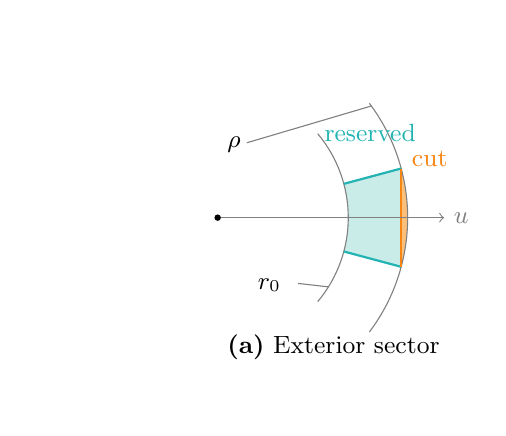
\begin{tikzpicture}[scale=1.16,font=\small]
 \fill[TealBlue!24] (15:1.43) arc (15:-15:1.43)
     -- (-15:2.08) arc (-15:15:2.08) -- cycle;
 \begin{scope}
  \clip (0,0) circle[radius=2.08];
  \fill[BurntOrange!48] (2.01,-.57) rectangle (2.12,.57);
 \end{scope}
 \draw[gray] (-40:1.43) arc (-40:40:1.43);
 \draw[gray] (-37:2.08) arc (-37:37:2.08);
 \draw[TealBlue,thick] (15:1.43)--(15:2.08) (-15:1.43)--(-15:2.08);
 \draw[BurntOrange,thick] (2.01,-.535)--(2.01,.535);
 \draw[->,gray] (0,0)--(2.48,0) node[right] {\(u\)};
 \fill (0,0) circle[radius=1pt];
 \node[anchor=west] at (0,.8) {\(\rho\)};
 \draw[gray] (.32,.82)--(36:2.08);
 \node[anchor=east] at (.8,-.74) {\(r_0\)};
 \draw[gray] (.88,-.72)--(-32:1.43);
 \node[TealBlue] at (1.67,.93) {reserved};
 \node[BurntOrange,anchor=west] at (2.02,.64) {cut};
 \node[anchor=west] at (0,-1.42) {\textbf{(a)} Exterior sector};
\end{tikzpicture}
\end{minipage}
\hfill
\begin{minipage}[t]{0.48\textwidth}
\centering
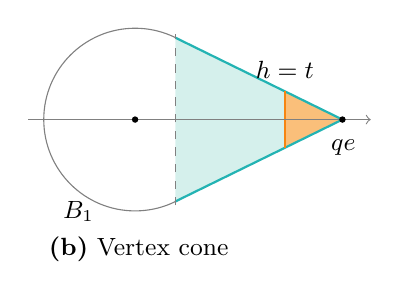
\begin{tikzpicture}[scale=1.16,font=\small]
 \draw[gray] (0,0) circle[radius=1];
 \fill[TealBlue!19] (.44,.897)--(2.27,0)--(.44,-.897)--cycle;
 \fill[BurntOrange!48] (1.64,.309)--(2.27,0)--(1.64,-.309)--cycle;
 \draw[TealBlue,thick] (.44,.897)--(2.27,0)--(.44,-.897);
 \draw[gray,dashed] (.44,-.94)--(.44,.94);
 \draw[BurntOrange,thick] (1.64,-.309)--(1.64,.309);
 \draw[->,gray] (-1.17,0)--(2.58,0);
 \fill (0,0) circle[radius=1pt] (2.27,0) circle[radius=1pt];
 \node[anchor=north] at (2.28,-.11) {\(qe\)};
 \node[anchor=south] at (1.64,.34) {\(h=t\)};
 \node[anchor=north] at (-.62,-.79) {\(B_1\)};
 \node[anchor=west] at (-1.05,-1.42) {\textbf{(b)} Vertex cone};
\end{tikzpicture}
\end{minipage}
\caption{Meridional sections, with radial gaps enlarged for clarity.
(a) Directions in a reserved sector avoid every inner cap. The
orange portion is the largest cap an exterior centre in that
direction can cut. (b) Beyond \(h=t\), the portion of the cone
from a selected vertex lies outside \(B_t\).}
\label{fig:annular-sectors}
\end{figure}
